\chapter{Software Process}
\label{chapter:SoftwareProcess}

An outstanding feature of ITK is the software process used to develop,
maintain and test the toolkit. The Insight Toolkit software continues to
evolve rapidly due to the efforts of developers and users located around the
world, so the software process is essential to maintaining its quality. If
you are planning to contribute to ITK, or use the Git source code repository,
you need to know something about this process (see
\ref{sec:ObtainingTheSoftware} on page \pageref{sec:ObtainingTheSoftware} to
learn more about obtaining ITK using Git). This information will help you
know when and how to update and work with the software as it changes. The
following sections describe key elements of the process.

\section{Git Source Code Repository}
\label{sec:GitRepository}

\index{ITK!Git repository}
\index{Git}

Git) is a tool for version control. It is a valuable resource for
software projects involving multiple developers.  The primary purpose
of Git is to keep track of changes to software. Git date and version
stamps every addition to files in the repository. Additionally, a user
may set a tag to mark a particular of the whole software. Thus, it is
possible to return to a particular state or point of time whenever
desired. The differences between any two points is represented by a
``diff'' file, that is a compact, incremental representation of
change. Git supports concurrent development so that two developers can
edit the same file at the same time, that are then (usually) merged
together without incident (and marked if there is a conflict). In
addition, branches off of the main development trunk provide parallel
development of software.

Developers and users can check out the software from the Git repository. When
developers introduce changes in the system,  Git facilitates to update the
local copies of other developers and users by downloading only the differences
between their local copy and the version on the repository.  This is an
important advantage for those who are interested in keeping up to date with the
leading edge of the toolkit. Bug fixes can be obtained in this way as soon as
they have been checked into the system.

ITK source code, data, and examples are maintained in a Git repository.  The
principal advantage of a system like Git is that it frees developers to try
new ideas and introduce changes without fear of losing a previous working
version of the software. It also provides a simple way to incrementally
update code as new features are added to the repository.

The ITK community use Git, and the Google web software tool Gerrit
(\url{http://review.source.kitware.com}) to facilitate a structured,
orderly method for developers to contribute new code and bug fixes to
ITK. The Gerrit review process allows anyone to submit a proposed
change to ITK, after which it will be reviewed by other developers
before being approved and merged into ITK.  For more information, see
\url{http://www.itk.org/Wiki/ITK/Git/Develop}.


\section{CDash Regression Testing System}
\label{sec:CDash}
\label{sec:QualityDashboard}

\index{Dashboard}
\index{Quality Dashboard}
\index{CDash}

One of the unique features of the ITK software process is its use of the CDash
regression testing system (\url{http://www.cdash.org}). In a
nutshell, what CDash does is to provide quantifiable feedback to developers as
they check in new code and make changes. The feedback consists of the results
of a variety of tests, and the results are posted on a publicly-accessible
Web page (to which we refer as a \emph{dashboard}) as shown in
Figure~\ref{fig:Dashboard}. The most recent dashboard is accessible from
\url{http://www.itk.org/ITK/resources/testing.html}). Since all users and developers of
ITK can view the Web page, the CDash dashboard serves as a vehicle for
developer communication, especially when new additions to the software is
found to be faulty.  The dashboard should be consulted before considering
updating software via Git.


\begin{figure}[ht]
\centering
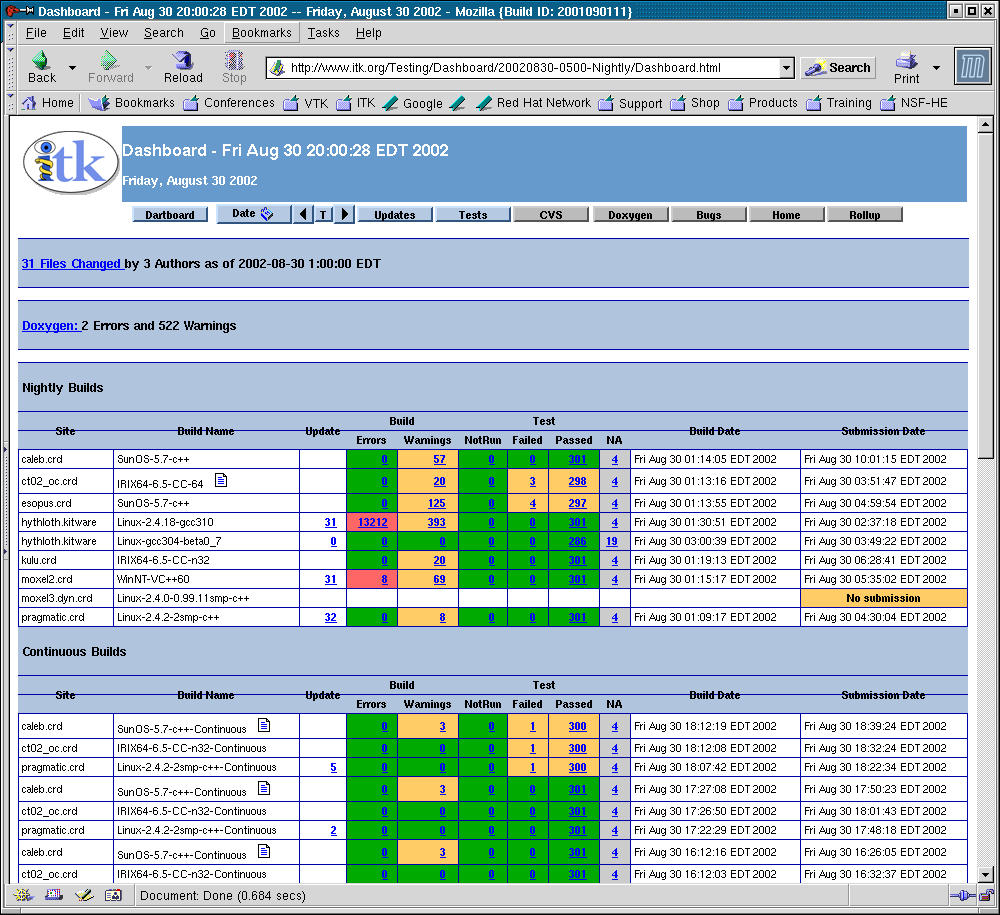
\includegraphics[width=0.7\textwidth]{Dashboard.eps}
\itkcaption[Dart Quality Dashboard]{On-line presentation of the quality
dashboard generated by CDash.}
\label{fig:Dashboard}
\end{figure}

Note that CDash is independent of ITK and can be used to manage quality
control for any software project. It is itself an open-source package and can
be obtained from

\begin{center}
\url{http://public.kitware.com/Dart/HTML/Index.shtml}
\end{center}

CDash supports a variety of test types. These include the following.
\begin{description}
        \item[Compilation.] All source and test code is compiled and linked.
        Any resulting errors and warnings are reported on the dashboard.

        \item[Regression.] Some ITK tests produce images as output. Testing
        requires comparing each test's output against a valid baseline image. If
        the images match then the test passes. The comparison must be
        performed carefully since many 3D graphics systems (e.g., OpenGL)
        produce slightly different results on different platforms.

        \item[Memory.] Problems relating to memory such as leaks, uninitialized
        memory reads, and reads/ writes beyond allocated space can cause
        unexpected results and program crashes. ITK checks run-time memory
        access and management using Purify, a commercial package produced by
        Rational. (Other memory checking programs will be added in the future.)

        \item[PrintSelf.] All classes in ITK are expected to print out all
        their instance variables (i.e., those with associated Set and Get
        methods) correctly. This test checks to make sure
        that this is the case.

        \item[Unit.] Each class in ITK should have a corresponding unit test
        where the class functionalities are exercised and quantitatively
        compared against expected results. These tests are typically written
        by the class developer and should endeavor to cover all lines of code
        including \code{Set/Get} methods and error handling.

       \item[Coverage.] There is a saying among ITK developers: \emph{If it
        isn't covered, then it's broke.} What this means is that
        code that is not executed during testing is likely to be wrong. The
        coverage tests identify lines that are not executed in the
        Insight Toolkit test suite, reporting a total percentage
        covered at the end of the test. While it is nearly impossible to
        bring the coverage to 100\% because of error handling code and similar
        constructs that are rarely encountered in practice, the coverage
        numbers should be 75\% or higher. Code that is not covered well enough
        requires additional tests.
\end{description}

Figure~\ref{fig:Dashboard} shows the top-level dashboard web page. Each row
in the dashboard corresponds to a particular platform (hardware + operating
system + compiler). The data on the row indicates the number of compile
errors and warnings as well as the results of running hundreds of
small test programs. In this way the toolkit is tested both at compile time
and run time.

When a user or developer decides to update ITK source code from Git it is
important to first verify that the current dashboard is in good shape. This
can be rapidly judged by the general coloration of the dashboard. A green
state means that the software is building correctly and it is a good day to
start with ITK or to get an upgrade. A red state, on the other hand, is an
indication of instability on the system and hence users should refrain from
checking out or upgrading the source code.

Another nice feature of CDash is that it maintains a history of changes to the
source code (by coordinating with Git) and summarizes the changes as part of
the dashboard. This is useful for tracking problems and keeping up to date
with new additions to ITK.

\section{Working The Process}
\label{sec:WorkingTheProcess}

The ITK software process functions across three cycles---the continuous
cycle, the daily cycle, and the release cycle.

The continuous cycle revolves around the actions of developers as they check
code into Git. When changed or new code is checked into Git, the CDash
continuous testing process kicks in. A small number of tests are performed
(including compilation), and if something breaks, email is sent to all
developers who checked code in during the continuous cycle. Developers are
expected to fix the problem immediately.

The daily cycle occurs over a 24-hour period. Changes to the source base made
during the day are extensively tested by the nightly CDash regression testing
sequence. These tests occur on different combinations of computers and
operating systems located around the world, and the results are posted every
day to the CDash dashboard. Developers who checked in code are expected to
visit the dashboard and ensure their changes are acceptable---that is, they
do not introduce compilation errors or warnings, or break any other tests
including regression, memory, PrintSelf, and Set/Get. Again, developers are
expected to fix problems immediately.

The release cycle occurs a small number of times a year. This requires
tagging and branching the Git repository, updating documentation, and
producing new release packages. Although additional testing is performed to
insure the consistency of the package, keeping the daily Git build error free
minimizes the work required to cut a release.

ITK users typically work with releases, since they are the most
stable. Developers work with the Git repository, or sometimes with periodic
release snapshots, in order to take advantage of newly-added features. It is
extremely important that developers watch the dashboard carefully, and
\emph{update their software only when the dashboard is in good condition
(i.e., is ``green'')}. Failure to do so can cause significant disruption if a
particular day's software release is unstable.

\section{The Effectiveness of the Process}
\label{sec:Effectiveness}

The effectiveness of this process is profound. By providing immediate
feedback to developers through email and Web pages (e.g., the dashboard), the
quality of ITK is exceptionally high, especially considering the complexity
of the algorithms and system. Errors, when accidently introduced, are caught
quickly, as compared to catching them at the point of release. To wait to the
point of release is to wait too long, since the causal relationship between a
code change or addition and a bug is lost. The process is so powerful that it
routinely catches errors in vendor's graphics drivers (e.g., OpenGL drivers)
or changes to external subsystems such as the VXL/VNL numerics library. All
of these tools that make up the process (CMake, Git, and CDash) are
open-source. Many large and small systems such as VTK (The Visualization
Toolkit \url{http://www.vtk.org}) use the same process with similar
results. We encourage the adoption of the process in your environment.

